\section{DDC Traffic Characterization}
\label{sec:workloads}
In this section, we characterize the network traffic workloads in disaggregated datacenters. We start by outlining the methodology in \S\ref{ssec:method1}. In \S\ref{ssec:flc}, we present results on network traffic characteristics in \dis, and compare these against the traffic characteristics in current server-centric datacenters. We close the section with a number of implications of our observations in \S\ref{ssec:knobs}.

\subsection{Methodology}
\label{ssec:method1} 
We use the same setup as in \S\ref{ssec:rmethod}, including the SIT, applications, datasets and cluster. The only difference is that we enabled the Virtual Private Network (VPC) in our cluster, ensuring no interference with other Amazon EC2 machines. 

\paragraphb{Capturing traffic in server-centric datacenters}
To characterize the network traffic in existing datacenters, we run the applications atop our EC2 cluster and capture the inter-machine traffic using {\tt tcpdump}~\cite{tcpdump}. {\tt tcpdump} gives us a packet-level log containing the five tuple for each packet. All packets with the same five-tuple constitute a single flow{\footnote{Applications choose one of the source ports randomly to establish a connection to the destination for each request. Given the large number of available ports, we assume that multiple connections between a pair of servers do not share the same port. However, memcached uses long-lived connections (all packets have the same five-tuple). In this case, we simply assumed each key-value pair lookup to be one flow.}}.

\paragraphb{Capturing memory and disk accesses}
At each individual server, we capture two types of traffic. First, application-level memory accesses using SIT (\S\ref{ssec:rmethod}) --- the request size in number of pages and the timestamp for each request into the server's main memory identified as ``remote memory'' ($75\%$ of main memory at the server since we use CPU local cache size to be $25\%$ (\S\ref{sec:requirements})). Second, application-level disk accesses using the {\tt blktrace} utility, which records a collection of (start\_block\_address, \#blocks, timestamp) tuples for each disk access request{\footnote{Note that a single application-level file request may generate multiple such records since the data residing on disk is not necessarily on consecutive disk blocks (due to disk fragmentation).}}. Since {\tt blktrace} trace is at the disk block granularity, identifying tuples corresponding to the same application-level request requires adding instrumentation to the application (which will impact traffic characteristics, \eg, flow arrival times). We instead assume that all tuples with timestamps within $50\mu$s constitute to the same application-level request. 

%
\begin{figure*}
  \centering
  \subfigure[Flow size distribution (\dis)]{
    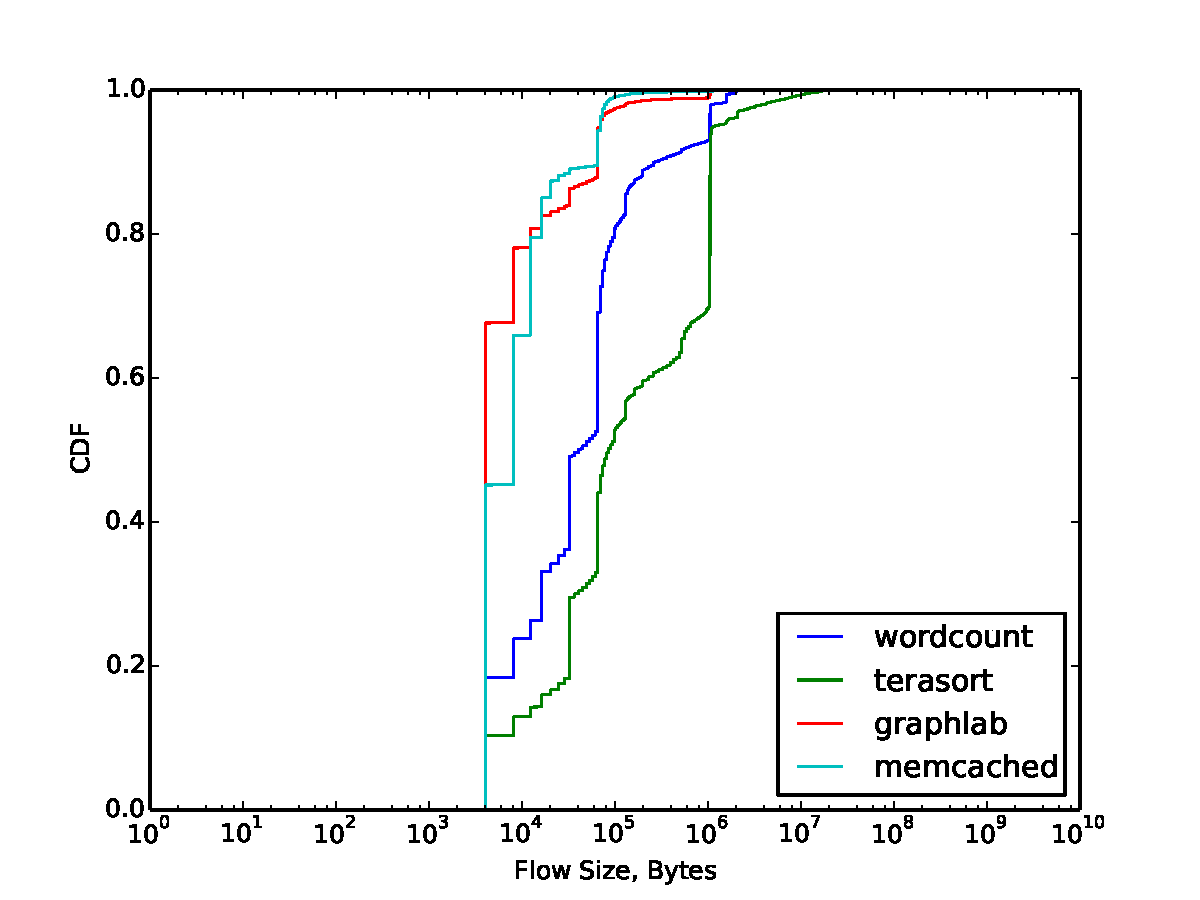
\includegraphics[width = 2in]{img/graph1_sizedist_dis} 
	\label{fig:fsd}
  }
%\hspace{0.05in}
  \subfigure[\#Flow in \dis and \pdis]{
    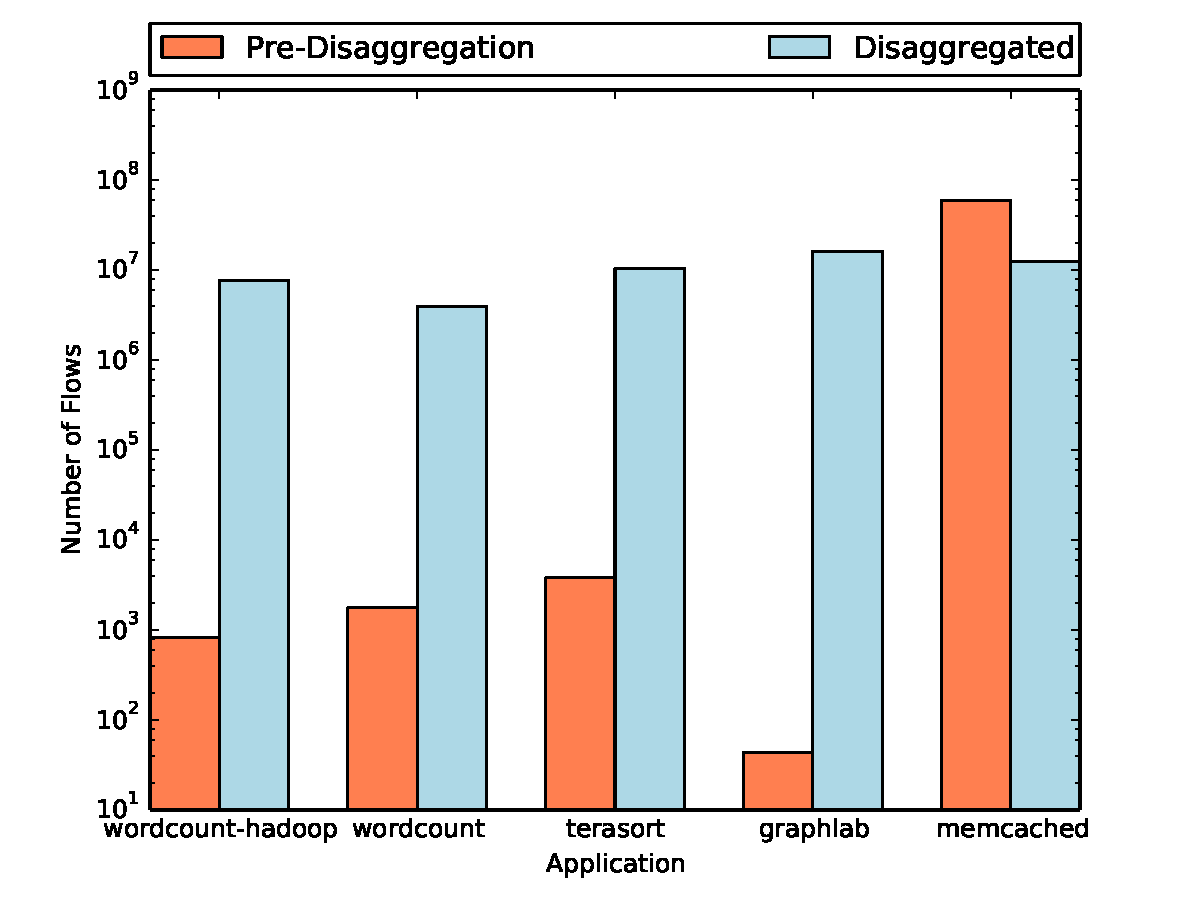
\includegraphics[width = 2in]{img/graph2_numflows}
	\label{fig:nof}
  }
  \subfigure[Temporal traffic distribution (\dis)]{
    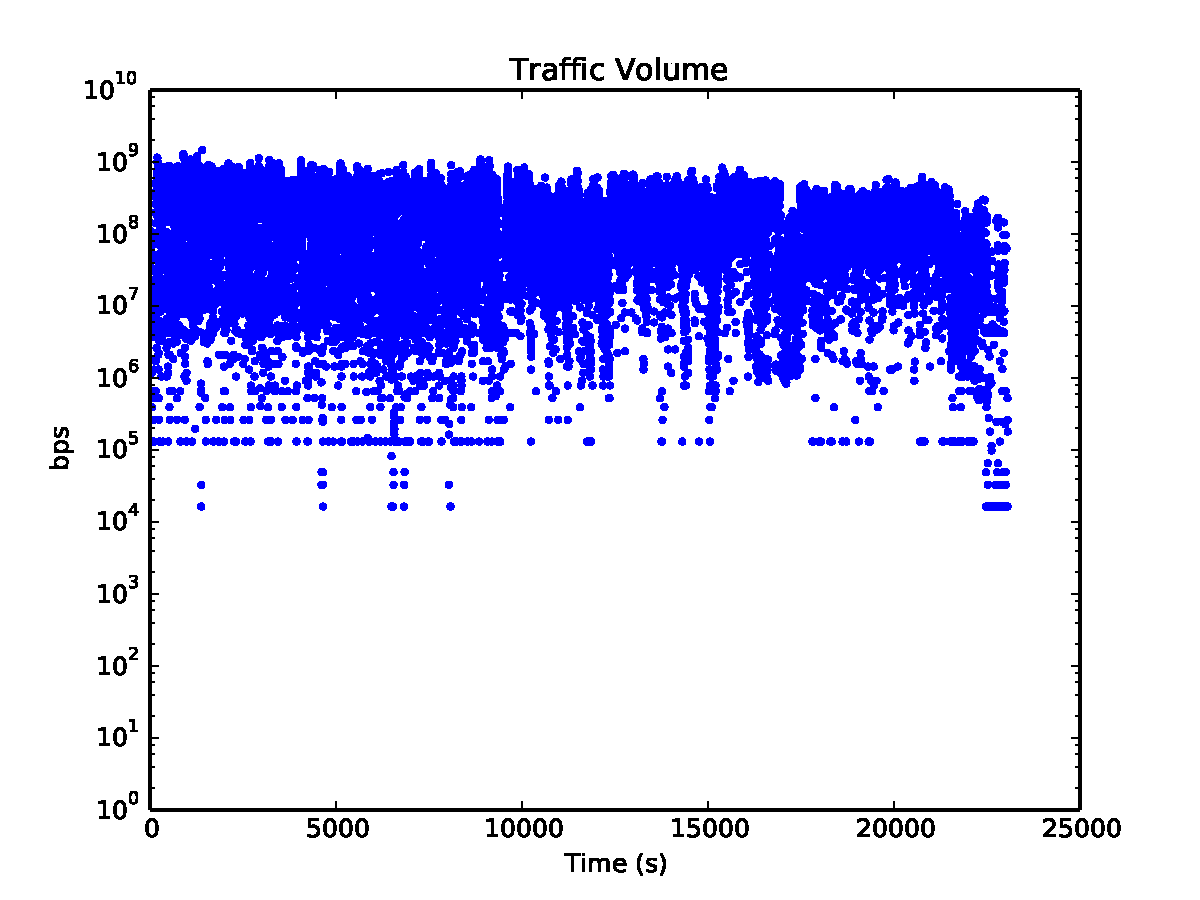
\includegraphics[width = 2in]{img/graph7_temporaltraffic_dis_terasort}
	\label{fig:ttd}
  }  
  \subfigure[Flow size distribution (\pdis)]{
    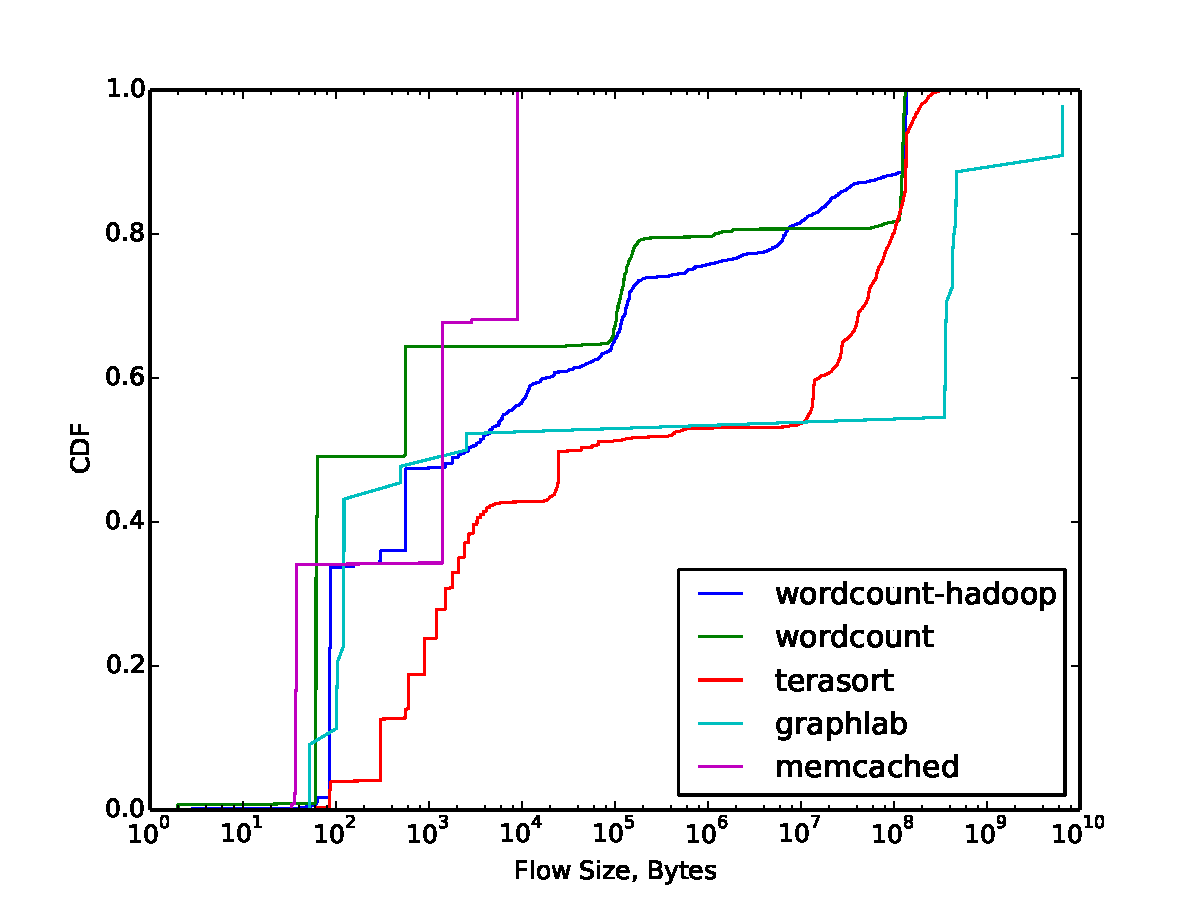
\includegraphics[width = 2in]{img/graph1_sizedist_pdis}
	\label{fig:fsdp}
  }
  \subfigure[Traffic volume in \dis and \pdis]{
    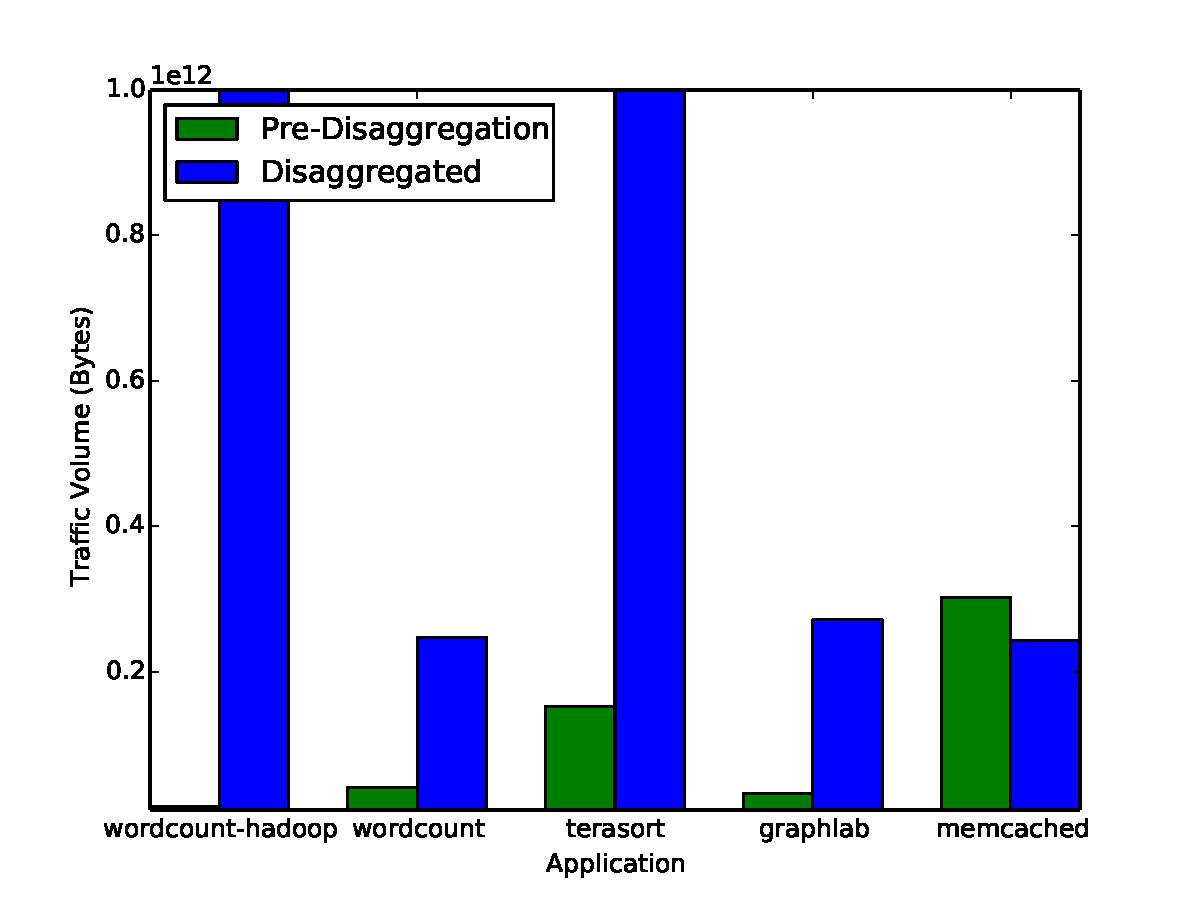
\includegraphics[width = 2in]{img/graph5_trafficvolume}
	\label{fig:tv}
  }  
  \subfigure[Temporal traffic distribution (\pdis)]{
    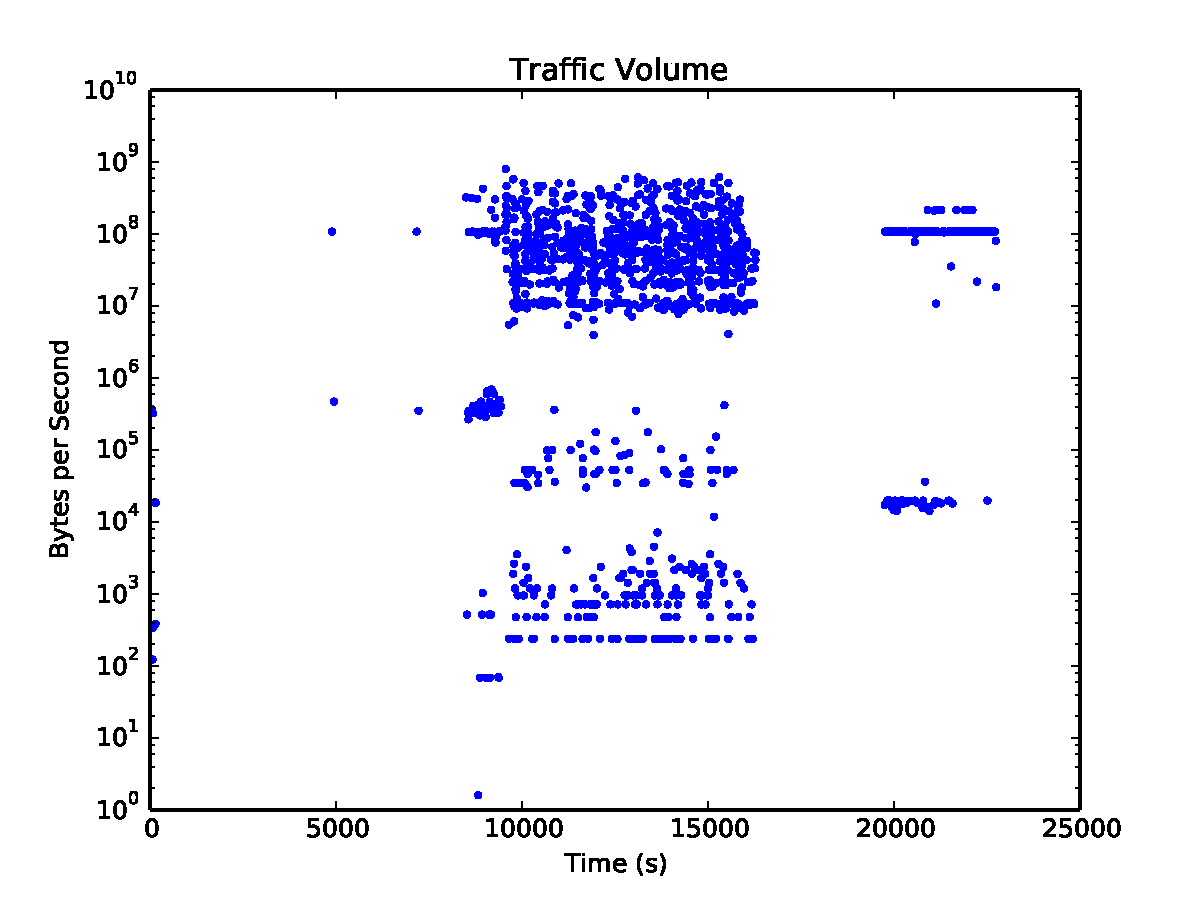
\includegraphics[width = 2in]{img/graph7_temporaltraffic_pdis_terasort}
	\label{fig:ttdp}
  }  
  \caption{\small{Flow and network traffic characteristics in \dis. Note that the x-axis is log-scaled for (a) and (d); the y-axis is log-scaled for all figures. \rc{Traffic volume is for terasort application}}}
  \label{fig:traffic}
\end{figure*}
%

The memory and disk requests using SIT and {\tt blktrace} are captured locally at each individual server. Some of these requests correspond to requests originating at remote CPUs (\eg, shuffle traffic). To correctly attribute requests to CPU that originates the request, we perform a timestamp-based matching between requests captured at each individual server, and inter-machine NIC traffic from {\tt tcpdump}. If a locally captured memory or disk access request matches to a NIC flow, it is assumed to be part of a remote read and is correctly attributed to the source of the NIC flow (more than $85\%$, on an average, were correctly attributed in our evaluation). Otherwise, the request is assumed to have been generated locally. 

\paragraphb{Data placement}
All memory and disk accesses captured above are associated with a specific address in the respective global virtual address space. This address space is partitioned across five memory blades and three disk blades{\footnote{Some of the disk space was not utilized in our cluster.}} in \dis using range partitioning. 
%for the entire address space nodes for a 5-machine ec2 cluster --- this represents the fact that disk access is slower than memory access, and thus can support more resource per blade without becoming bandwidth constrained.
In particular, the address space for memory and disk on each individual server is partitioned into five and three parts, respectively, to match the number of resource blades. Each range is then mapped to one of the blades. Note that, as discussed in \S\ref{ssec:system}, this mapping enables distributed data placement since a memory or disk access in our EC2 cluster may now be mapped along multiple blades.

\paragraphb{Transforming accesses into network flows}
The above methodology provides us the amount of data accessed and the corresponding timestamps for each pair of CPU-memory and CPU-disk blades in \dis (memory-disk blades to not communicate directly). For any pair of resource blades, we transform access requests into network flows by combining requests with timestamps within $50\mu$s into a single flow.  Finally, a read request on disk and memory blades is considered a flow with corresponding blade being the source and CPU being the destination; write requests are considered as flows in the opposite direction.

\subsection{Traffic Characterization} 
\label{ssec:flc}
We discuss the traffic characteristics in \dis, and contrast them against the traffic in existing server-centric datacenters.

\paragraphb{Flow Sizes and number of flows} 
Figure~\ref{fig:fsd} and Figure~\ref{fig:fsdp} show the flow size distribution for \dis and for existing datacenters. Note that the flow size distribution for existing datacenters closely resembles the distribution observed in previous studies~\cite{srikanth, theo}. We observe that, in a sharp contrast to current datacenters, the flow sizes in \dis are concentrated in a small range [4KB, 40MB] --- two orders of magnitude smaller for the long flow sizes in current datacenters. Intuitively, two factors contribute to the differences. First, as outlined in \S\ref{ssec:rmethod}, the granularity of remote traffic in \dis is eith a page size ($4$KB) or a disk block size ($4$KB) leading to lack of short flows. Second, distributed data placement in \dis (\S\ref{ssec:rmethod}) distributes long flows along multiple CPU-disk blade pairs, reducing the tail in flow size distribution.

Figure~\ref{fig:nof} shows that the number of flows in \dis increases by $3$--$4$ orders of magnitude compared to server-centric datacenters (except for memcached, discussed below). This is not surprising since the disk and memory flows that are contained within a single server in existing datacenters are not injected into the network fabric. The case of memcached is rather interesting since the number of flows in \dis decreases when compared to server-centric datacenters. Indeed, in a five server cluster running memcached in current datacenters, every one out of five client requests are going to be injected into the network (since the desired data is cached on a remote server). In \dis with $25\%$ local cache, CPU blades can respond to $25\%$ of the requests locally and only $75\%$ of the requests are going to be injected into the network.

found that while in \pdis each request will result in a network flow, in \dis some requests are serviced by the local memory cache without crossing the network. This phenomenon is discussed further in~\S\ref{sssec:tfvol}.

%Second, across all the applications we evaluated, the flow size distribution is dominated by memory traffic (4KB flows) and at least $60\%$ of the flows are less than $100$KB. 

 results to discuss:
\begin{itemize}
\item The flow size distribution in \dis is more homogeneous --- that is, compared to \pdis, flows are distributed over a smaller range. \rc{flow sizes concentrated within a smaller range}
\item For most applications, both the number of flows and the overall traffic volume in \dis are greater than the number of flows in \pdis. \rqc{\#flows increase by 3-4 orders of magnitude, but volume only by 2}
\item \rqc{handling the increased traffic volume does not require 2 orders of magnitude more bandwidth --- peak traffic volume does not change}
\item \rqc{rather non-intuitively, applications executing in-memory point queries require fewer flows and volume} 
\item While in \pdis the traffic volume is spread over all source-destination pairs, in \dis a number of such pairs have no traffic between them --- that is, the traffic matrix changes from all-to-all to some-to-some.
\item \rqc{stuff from yet-to-be-written 4.4}
\end{itemize}
%

\paragraphb{Traffic volume}
\label{sssec:fctv}


\rc{This section along with figure 8 are slated for removal because we cannot count remote memory flows.}
Next, we study the flow arrival times in \dis. Figure~\ref{fig:fat} shows the flow arrival time distribution for the six applications from Table~\ref{tab:workloads}. We make two interesting observations. First, the flow arrival time distribution is essentially independent of the application. This is because memory access traffic dominates all the applications, leading to similar flow arrival time distribution. Second, the flow arrival time distribution is significantly different from Poisson distribution, a commonly accepted approximation to workloads in \pdis. \rc{We should say something about inter-flow arrival times --- too small? not too small? any significant different compared to \pdis?}

Figure~\ref{fig:fat} also shows the flow arrival time distribution in \pdis. As observed in several previous studies~\cite{srikanth, theo}, the distribution is very close to Poisson distribution providing a second order support to our evaluation methodology. In comparison to \pdis, the distribution is significantly different in \dis as discussed above.

We start with studying the traffic volume in \dis and \pdis (see Figure~\ref{fig:vol}). For most applications studied, the traffic volume in \dis increases due to the same reason the number of flows increases (shown in Figure~\ref{fig:nof}) --- intuitively, flows that previously were contained within a server are now carried over the network.

Just as memcached exhibits a greater number of flows in \pdis, its traffic volume is greater in \dis. Our experiments with 25\% of memory in the local cache, so we expect that approximately this amount of request traffic in memcached will be served from the local cache in \dis and avoid the network entirely. Accordingly, we observe that the difference in traffic volume between \dis and \pdis is 24\%. The difference in the number of flows is more drastic because the flow distributions are different --- while memcached in \pdis has a bimodal distribution of request and response flows of approximate size 30 bytes and 10KB respectively, in \dis the distribution varies in the range [4KB, 19MB]. The longer tail in flow sizes for \dis causes the drastic disparity in number of flows seen in Figure~\ref{fig:nof} despite a relatively modest increase in traffic volume.

% We note that the traffic volume in \dis is not much larger than in \pdis. At the first glance, this may seem rather surprising given the increase in traffic due to intra-server traffic becoming remote. However, note that memory accesses are just $4$KB in size; thus, a significantly large number of memory access traffic will correspond to a single long flow. Moreover, reads and writes that are local are only increased by a factor of $2\times$.

\begin{figure}[t]
  \centering
  \subfigure{
    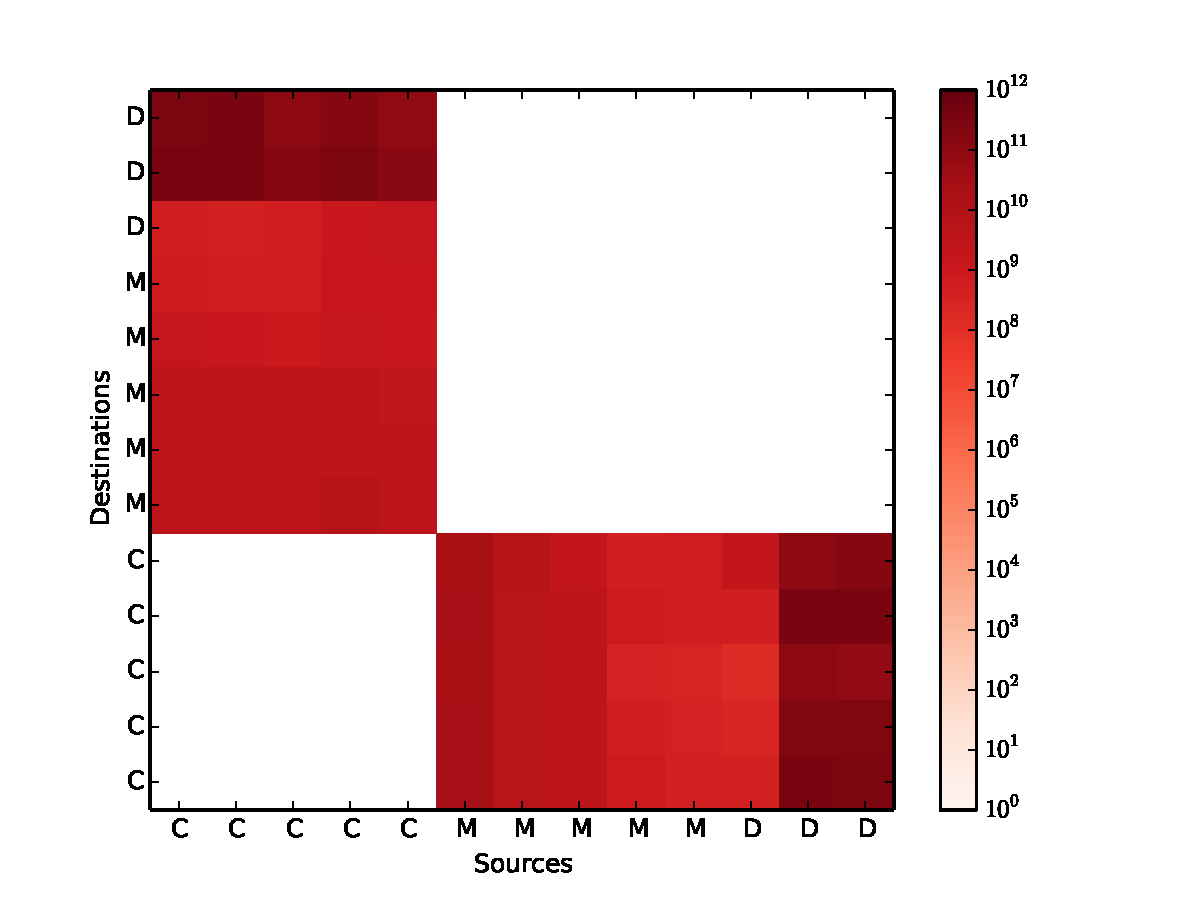
\includegraphics[width = 2.3in]{img/graph6_trafficvolumeheatmap_dis_terasort} 
	\label{fig:asdd}
  }
%\hspace{0.05in}
  \subfigure{
    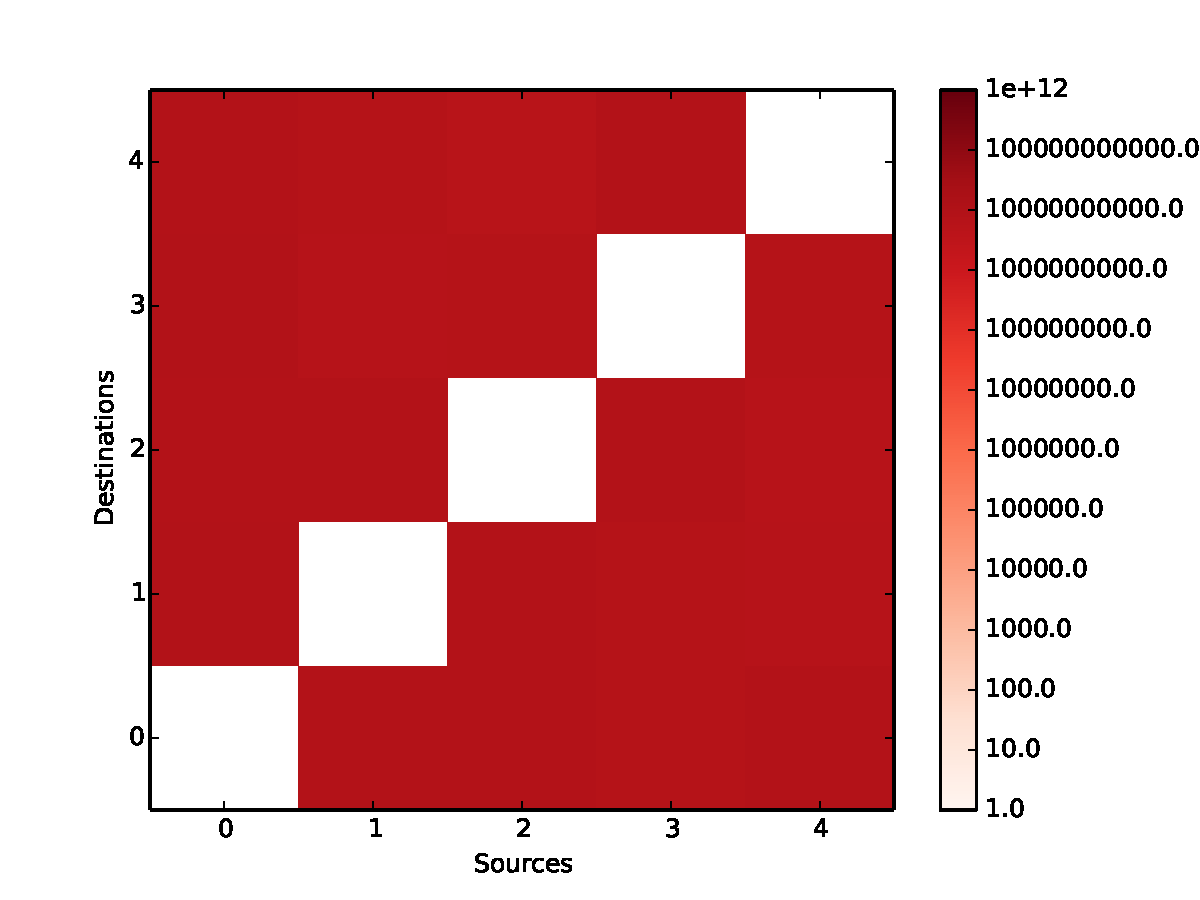
\includegraphics[width = 2.3in]{img/graph6_trafficvolumeheatmap_pdis_terasort}
	\label{fig:sdds}
  }
  \caption{\small{Spatial traffic distribution in \pdis and \dis for the terasort application. The x-axis represents senders and the y-axis receivers. In \pdis above, this is a $5 \times 5$ matrix for the 5 ec2 machines, while in \dis below, the heatmap is a $13 \times 13$ matrix, for the 5 cpu blades, 5 memory blades, and 3 disk blades we map the 5 ec2 machines to. For further details on this mapping see \S\ref{ssec:method1}.}}
  
  %A $n \times n$ matrix heat diagram, with cell $(i, j)$ having heat level corresponding to the traffic volume between source i and destination j. The same thing for \pdis.}}}
  \label{fig:sd}
\end{figure}
%
\paragraphb{Temporal and Spatial distribution}
We now study the spatial distribution of traffic in \dis (see Figure~\ref{fig:sd}). Note that all traffic represented in Figure~\ref{fig:sdds} has a CPU as either its source or destination. This is a consequence of our assumption as discussed in \S~\ref{sec:summary} that CPUs do not share memory or disk resources. One could however imagine alternate models in which not all traffic is CPU-based. For example, disk accesses could be sent to the CPU that requested them while simultaneously being cached in remote memory. We leave an exploration of this design space to future work.

Also note that there are slightly more traffic volume to the first memory blades than to memory blades farther rightwards and upwards in the heatmap. Digging deeper, we found that lower memory addresses were more popular in the application shown, terasort\footnote{results for other applications are in Appendix ~\ref{sec:appendix}}. As a result, the memory blade that lower addresses were mapped to in our range hashing experienced a greater traffic volume from CPUs. This suggests that depending on the application's data access patterns, a different address mapping may be needed.
%First, when compared to \pdis, the traffic in \dis is significantly well distributed across the source-destination pairs. Indeed, the \dis architecture allows distributing a single read/write traffic across multiple nodes spatially distributed across the network. Second, the overall spatial distribution in \dis has significantly lower temperature than in \pdis, implying that on an average, each source-destination pair observes significantly lower traffic volume in \dis when compared to \pdis.

Finally, we study the temporal distribution of traffic in \dis and \pdis. Figure~\ref{fig:td} shows that, when compared to \pdis, the traffic distribution in \dis is significantly less bursty. This is because of an interesting effect caused by the data placement discussed in \S\ref{sec:summary}. When a long flow in \pdis is divided across multiple smaller flows in \dis (due to data placement across multiple disks), it is pipelined into multiple shorter flows. Akin to the task packing problem, where having multiple smaller tasks has a better packing compared to a single long task, dividing a single flow into multiple smaller flows ``packs'' into the network more efficiently, making traffic less bursty.

\subsection{Implications}
\label{ssec:knobs}

We now study how various design parameters in \dis architecture design impact the observations made in this section. 

% \paragraphb{Impact of cache size} % discussed in section 3.
%\begin{figure}[t]
%\centering
%\subfigure{
%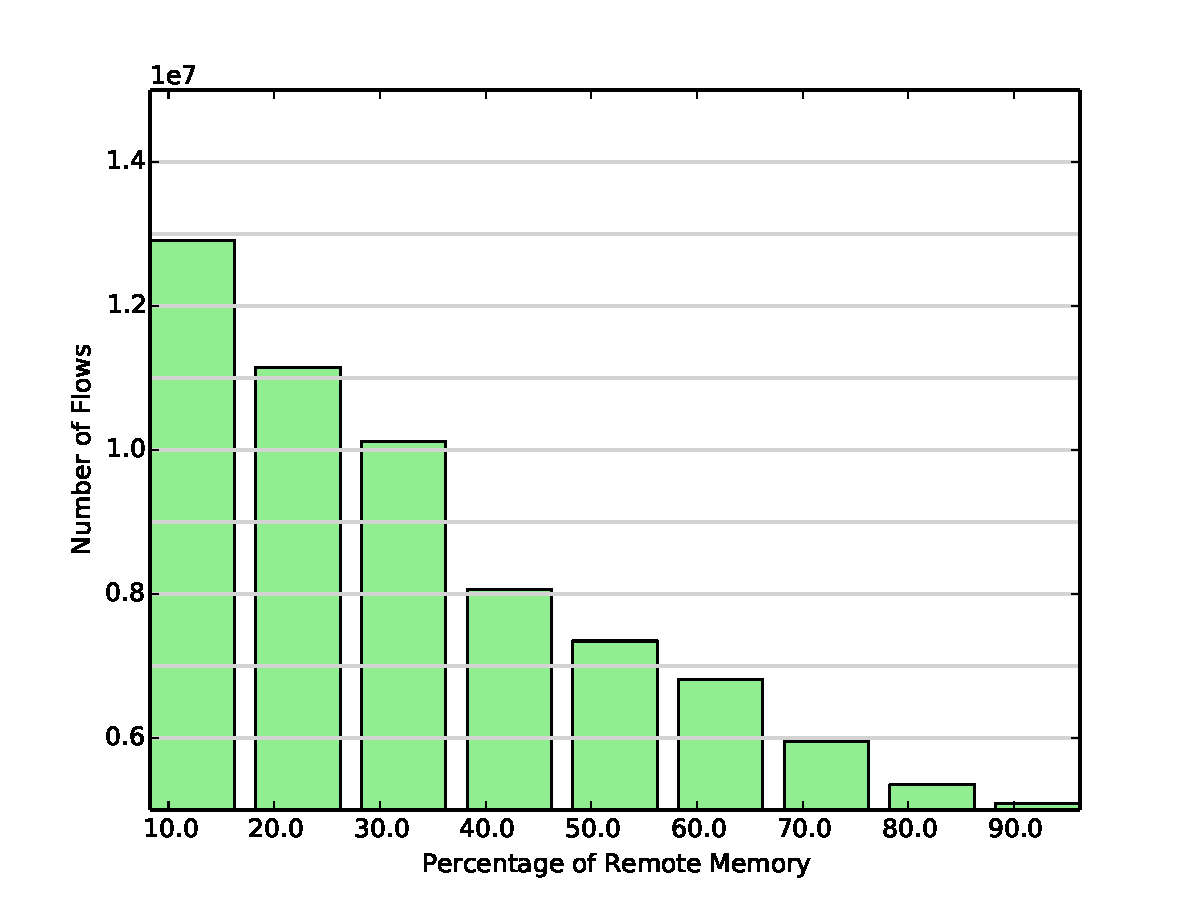
\includegraphics[width = 3.0in]{img/rmem_numflows}
%\label{fig:rmem_numflows}
%}
%\subfigure{
%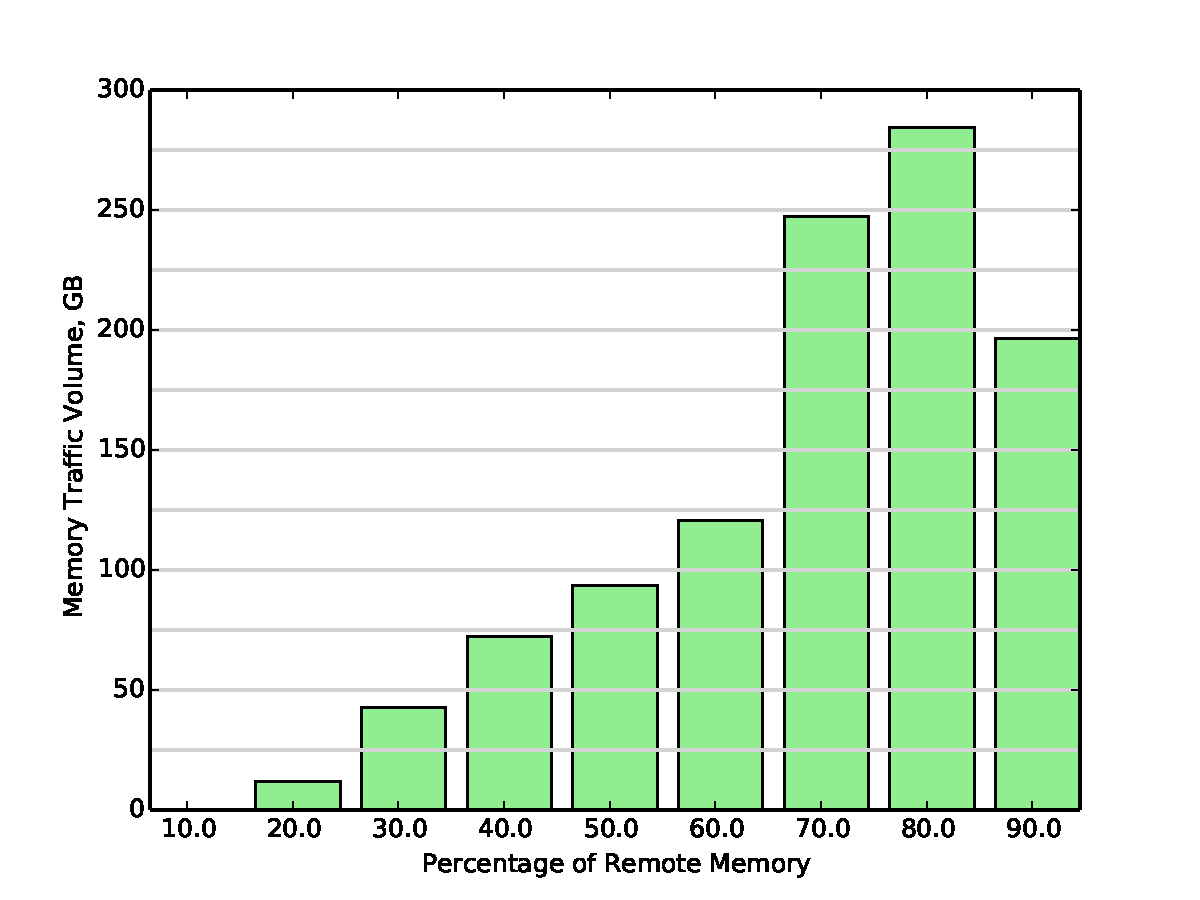
\includegraphics[width = 3.0in]{img/rmem_trafficvolume}
%\label{fig:rmem_trafvol}
%}
%\caption{Flow count (above) and traffic volume (below) with varying fraction of memory in the local cache.}
%\label{fig:rmem}
%\end{figure}

\paragraphb{Impact of remote versus local} 
\rqc{Peter's graphs showing performance of local disk vs remote memory}

\rc{what do these mean?}
    
\paragraphb{Impact of disaggregation scale}

\paragraphb{Impact of data placement}

\subsubsection{Implications}
Our characterization of flows in \dis allows us to draw two conclusions. First, given that \dis traffic is dominated by latency-sensitive short flows and that the number of flows increases dramatically, centralized solutions to flow scheduling may not be practical. Such solutions, if deployed in \dis, would need to dramatically lower short-flow latency as well as be able to scale up to cope with larger numbers of flows. Second, future protocols should be designed with our flow characteristics in mind --- namely, protocols should not rely on the elephant-mice conjecture for performance, and should be able to handle a more homogeneous flow size distribution. \rqc{more implications?}

\begin{itemize}[leftmargin=*]
	\itemsep0em
	\item Traffic dominated by latency-sensitive short flows --- centralized flow schedulers may be inefficient
	\item Number of flows increased --- centralized solutions may see more scalability issues
	\item \rc{slated for removal} Flow arrival times too small --- centralized solutions inefficient
	\item More homogeneity in flow sizes --- design of protocols
	\item Traffic volume more uniformly distributed across short and long flows --- design of protocols
\end{itemize}


\subsubsection{Implications}
\label{ssec:implications}
\rc{Is this a valid implication?}
Overall, while we observed in \S\ref{sec:requirements} that low latencies are important for performance, we observe here that high bandwidths are not necessary to serve the volume of traffic injected into the network. Rather, we envision networks in \ddc being provisioned to meet \emph{latency} requirements, and being overprovisioned from a peak traffic volume perspective as a result. \rqc{more implications?} 

%\begin{itemize}[leftmargin=*]
%	\itemsep0em
%	\item Traffic volume --- do not need very high bandwidth networks
%	\item Spatial distribution --- traffic not so local
%	\item Temporal distribution --- do not need to design networks for peak traffic?
%\end{itemize}	

%Our range hashing works as follows: 
%\begin{enumerate}
%\item the address space for each node is split evenly into (number of nodes) contiguous ranges --- memory space split into 5 and disk space split into 3
%\item each range is mapped to one disaggregated node
%\item this is done for all five ec2 machines
%\item Using a range hashing algorithm allows for sequential address accesses to be pipelined for higher throughput. 
%\item We leave a more thorough exploration of this particular design knob to future work.
%\end{enumerate}

%
% \begin{figure}
% 	\centering
% 	\begin{tikzpicture}[xscale=0.5, yscale=0.35]

% 	\draw[very thick, black, <->] (-1, 12.25) to [out=45, in=135] (5, 12.25);

% 	\draw[thick, fill=white] (-3, 5) rectangle (1, 11); 
% 	\draw[thick, fill=white] (-2, 12) rectangle (0, 10); 
% 	\draw (-1, 11) node {\small{CPU}};
% 	% \draw (-1, 10.5) node {\small{Handler}};
	
% 	\draw[thick, fill=blue] (-2.75, 7.5) rectangle (-0.75, 8.5);
% 	\draw[thick, fill=green] (-2.75, 5.5) rectangle (-0.75, 7.5);
% 	\draw (-1.75, 8) node {\small{LM}};
% %	\draw (-2.75, 7.5) -- (-0.75, 7.5);
% 	\draw (-1.75, 6.5) node {\small{RM}};
% %	\draw (-2.75, 6.5) -- (-0.75, 6.5);
% %	\draw (-1.75, 6) node {\small{K$\to$O}};

% %	\draw[thick] (-0.25, 5.5) rectangle (0.75, 8.5);
% 	\draw[thick, fill=gray] (-0.25, 8.5) rectangle (0.75, 7.5);
% 	\draw[thick, fill=gray] (-0.25, 5.5) rectangle (0.75, 6.5);
% 	\draw (0.25, 7) node {\small{$\dots$}};

% 	\draw[very thick, black, dashed, <->] (-1.5, 10) -- (-1.75, 8.5);
% 	\draw[very thick, black, dashed, <->] (-0.5, 10) -- (0.25, 8.5);
% 	\draw[very thick, black, dashed, <->] (-0.5, 10) -- (-0.45, 6);

% 	\draw (2, 6.5) node {\Large{$\dots$}};

% 		\draw[thick, fill=white] (3, 5) rectangle (7, 11); 
% 		\draw[thick, fill=white] (4, 12) rectangle (6, 10); 
% 		\draw (5, 11) node {\small{CPU}};
% 		% \draw (5, 10.5) node {\small{Handler}};

% 		\draw[thick, fill=green] (3.25, 5.5) rectangle (5.25, 7.5);
% 		\draw[thick, fill=blue] (3.25, 7.5) rectangle (5.25, 8.5);
% 		\draw (4.25, 8) node {\small{LM}};
% 		\draw (4.25, 6.5) node {\small{RM}};

% 	%	\draw[thick] (-0.25, 5.5) rectangle (0.75, 8.5);
% 		\draw[thick, fill=gray] (5.75, 8.5) rectangle (6.75, 7.5);
% 		\draw[thick, fill=gray] (5.75, 5.5) rectangle (6.75, 6.5);
% 		\draw (6.25, 7) node {\small{$\dots$}};

% 		\draw[very thick, black, dashed, <->] (4.5, 10) -- (4.25, 8.5);
% 		\draw[very thick, black, dashed, <->] (5.5, 10) -- (6.25, 8.5);
% 		\draw[very thick, black, dashed, <->] (5.5, 10) -- (5.55, 6);

% 	\end{tikzpicture}
% 	    \caption{\small{We run real-world applications on a $5$-node Amazon EC2 cluster and emulate disaggregated architecture as follows. The memory accesses are captured into ``local cache'' accesses and ``remote memory'' accesses using an in-house implementation of a special instrumentation tool (SIT) described in \S\ref{sec:workloads}. The local disk accesses are captured using the {\tt blktrace} utility. Finally, all remote memory and disk accesses are captured using {\tt TCPdump}.}}
% 	\label{fig:system2}
% \end{figure}
%

%However, this would require changes in the application, and possibly in network elements at the end hosts. To avoid such complications, we simply assume that each remote memory access and disk access constitutes a flow in disaggregated datacenter.

% \paragraphb{Limitations}
% Our instrumentation approach has two significant limitations. First, access to memory and disk accesses is only possible at page and block granularity, respectively. While we cannot explore other points in this design space, as discussed in \S\ref{sec:summary} page and block level accesses in \dis are a reasonable granularity at which to structure remote accesses in \dis. Second, accesses caused by remote flows and accesses that originated locally are indistinguishable, and thus we use a heuristic to assign disk flows to remote CPU nodes. However, we note this limitation affects only the assignment of flows to source-destination pairs, not the amount of traffic observed.

%\begin{enumerate}
%\item Our instrumentation only allows access to memory and disk accesses at page and block granularity, respectively. While as discussed earlier page-level accesses may be desirable in \dis for locality, we were unable to explore other points in the design space.
%\item Our instrumentation cannot distinguish between accesses caused by remote flows and accesses that originated locally. We are forced to use a heuristic to assign disk flows to remote CPU nodes.
%\end{enumerate}

%
%
% \begin{figure}
%   \centering
%     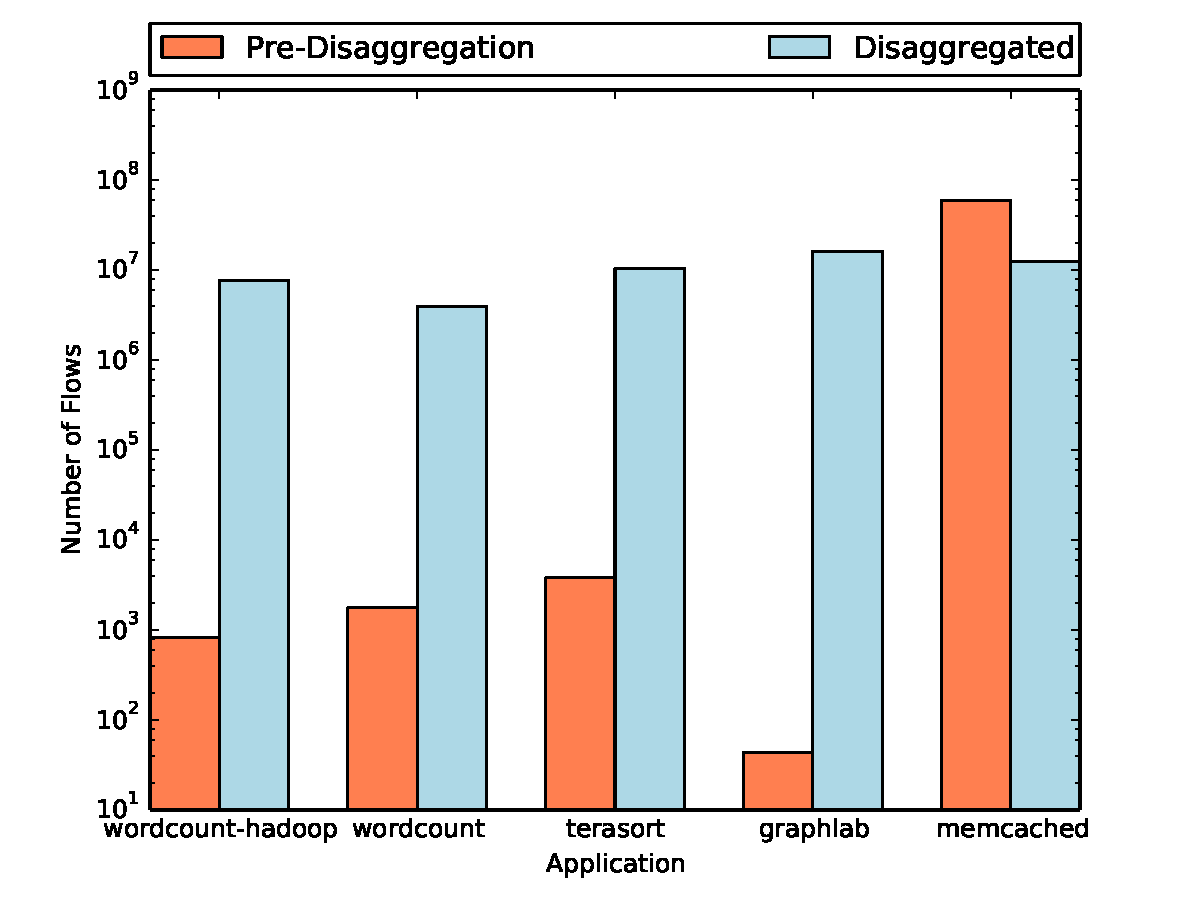
\includegraphics[width = 2.5in]{img/graph2_numflows} 
%   \caption{\small{Number of flows in \dis and \pdis. Note that the y-axis is log-scaled.}}
%   \label{fig:nof}
% \end{figure}
%
%
%Figure~\ref{fig:vof} shows that the number of bytes in \dis is more uniformly distributed across short and long flows when compared to \pdis. There are two main reasons for this -- the memory flows dominating the network flows (thus having more bytes in short flows), and the long flows having been distributed across the network leading to reduction in \#bytes in long flows \rc{$\gets$ not sure about this}
%
% \begin{figure}
%   \centering
%   \subfigure{
%     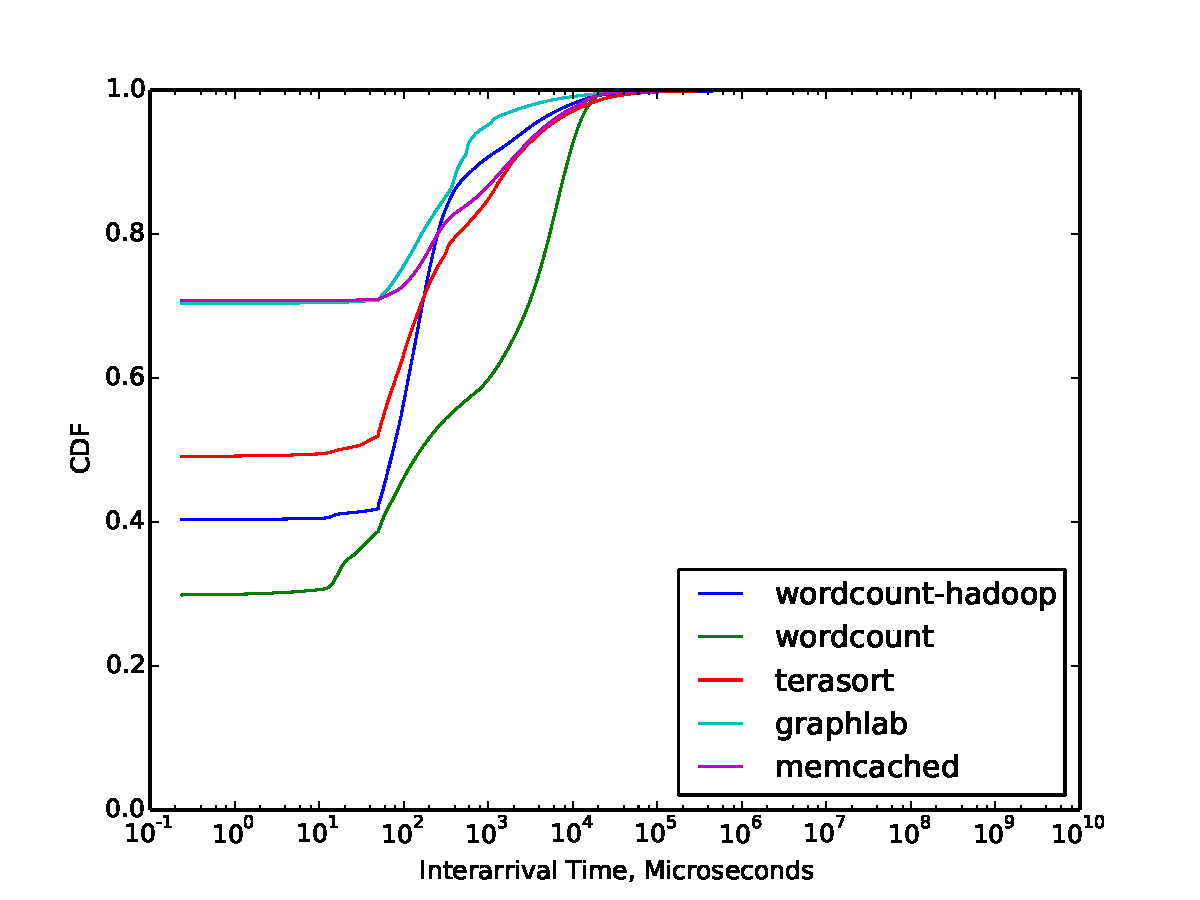
\includegraphics[width = 2.3in]{img/graph4_interdist_dis} 
% 	\label{fig:asdd}
%   }
% %\hspace{0.05in}
%   \subfigure{
%     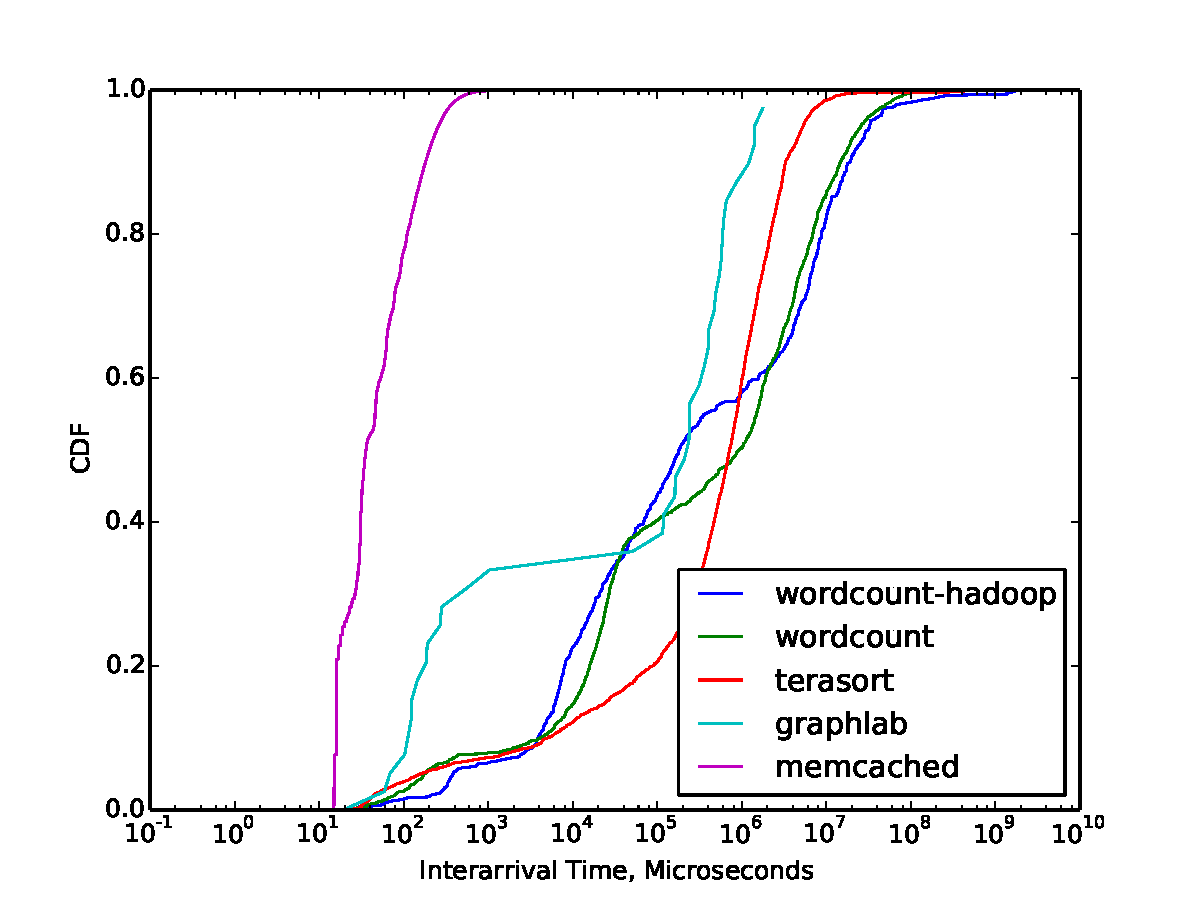
\includegraphics[width = 2.3in]{img/graph4_interdist_pdis}
% 	\label{fig:sdds}
%   }
%   \caption{\small{Flow arrival time distribution in \dis and \pdis. All the applications go into one figure: six lines in the CDF, one for each application. The same thing for \pdis. \rc{if figure stays look at graphlab going to 1}}}
%   \label{fig:fat}
% \end{figure}
%
%
%
% \begin{figure}
%   \centering
%     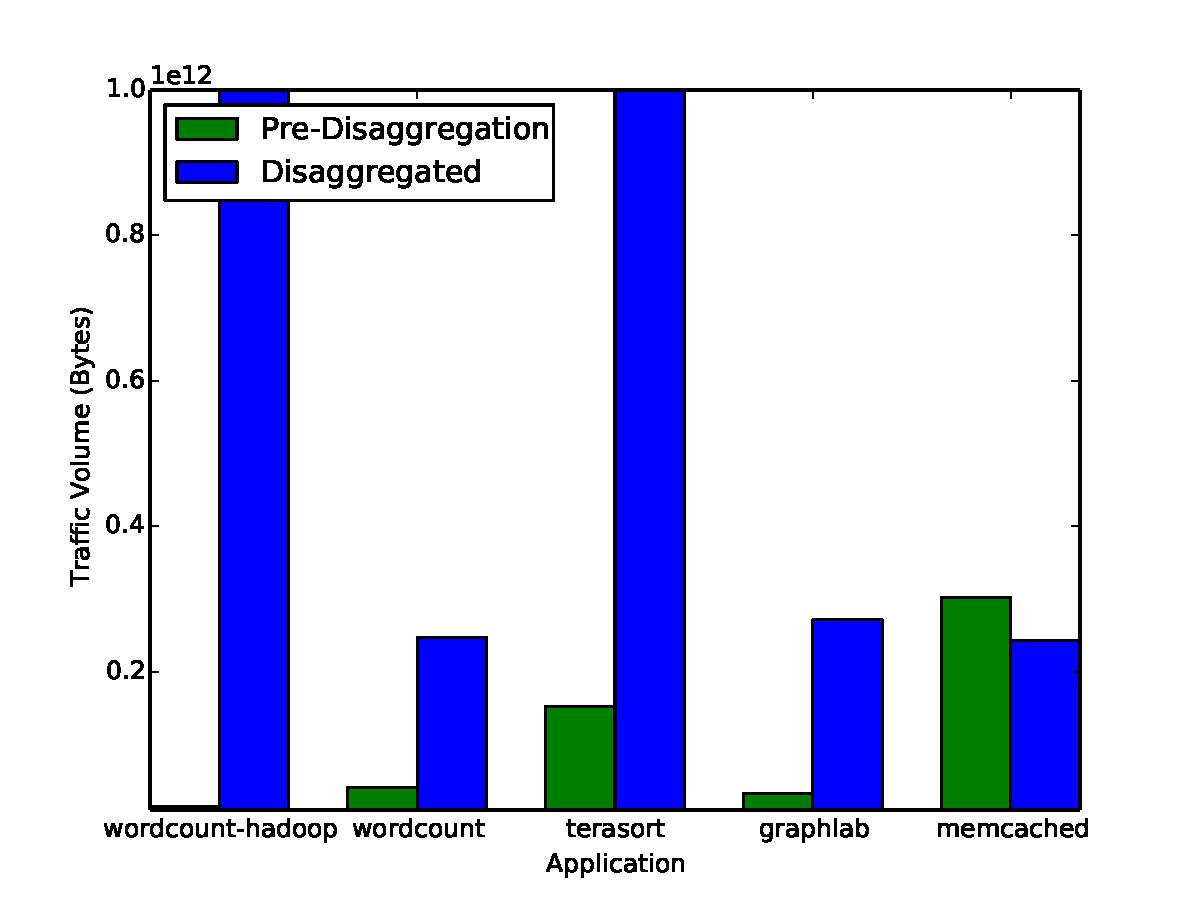
\includegraphics[width = 2.5in]{img/graph5_trafficvolume} 
%   \caption{\small{Traffic volume in \dis and \pdis. Note that the y-axis is log-scaled.}}
%   \label{fig:vol}
% \end{figure}
%
% \begin{figure}[t]
%   \centering
%   \subfigure{
%     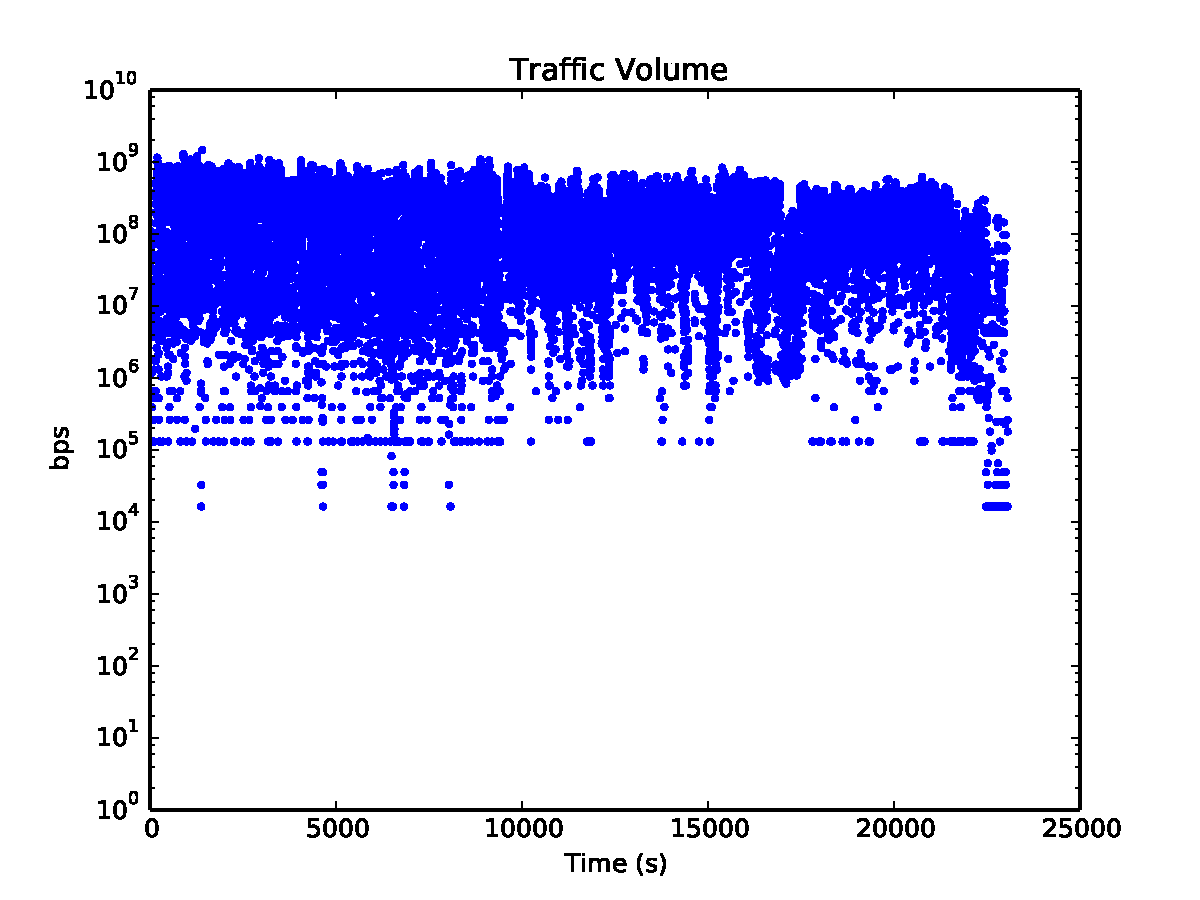
\includegraphics[width = 2.3in]{img/graph7_temporaltraffic_dis_terasort} 
% 	\label{fig:asdd}
%   }
% %\hspace{0.05in}
%   \subfigure{
%     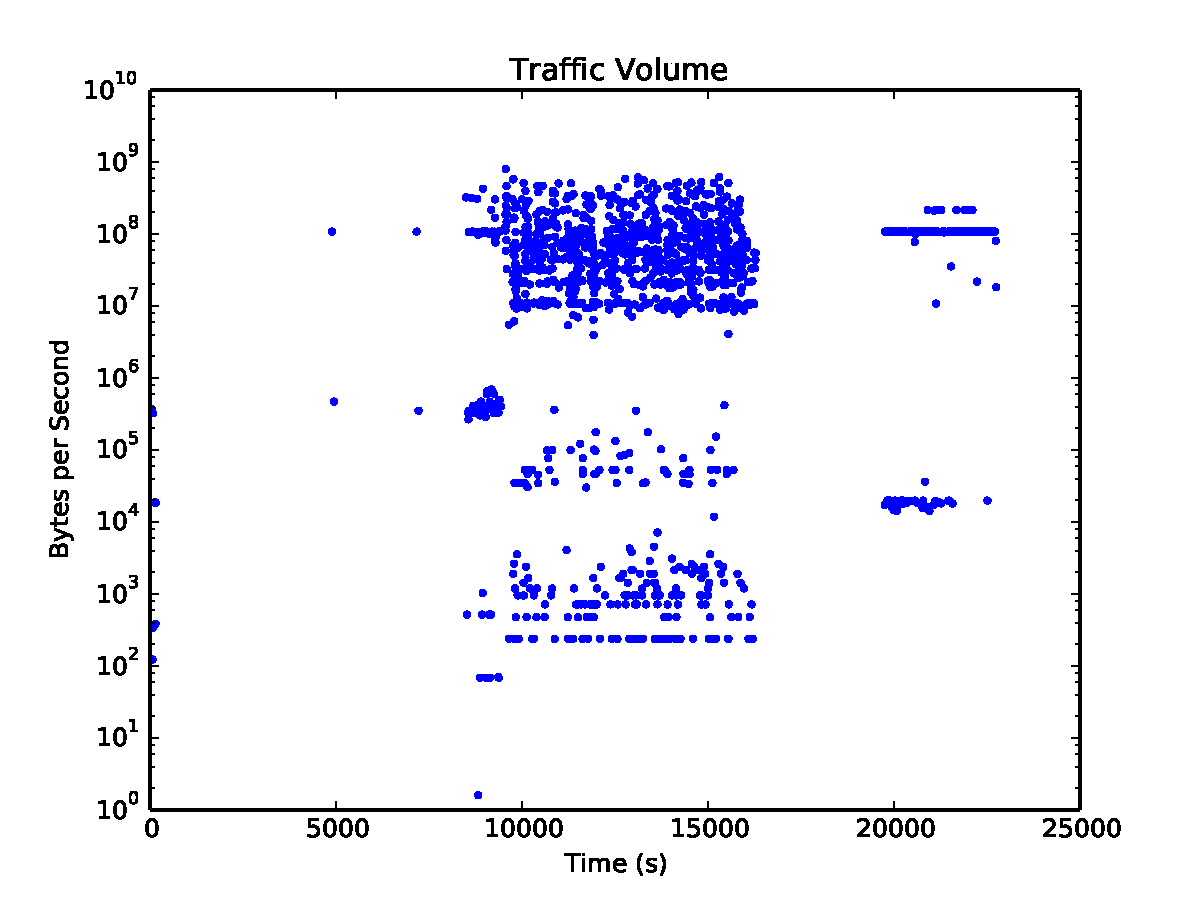
\includegraphics[width = 2.3in]{img/graph7_temporaltraffic_pdis_terasort}
% 	\label{fig:sdds}
%   }
%   \caption{\small{Temporal traffic distribution in \dis and \pdis for one of the applications. The trace was divided into 100ms timeslots, and flows were assigned to slots based on their start time. The traffic volume in these timeslots was then normalized to determine a value in bytes per second. Note the y-axis is log-scale.}}
%   \label{fig:td}
% \end{figure}
%